\section{Durchführung}
\label{sec:Durchführung}

\subsection{Versuchsaufbau}

In dem Versuchsaufbau ist wie in \autoref{sec:nachweis} bereits beschrieben eine evakuierte Photozelle
mit einem Picoamperemeter und einer variablen Spannungsquelle verbunden.
Für die Bestrahlung der Photokathode wird eine optische Konstruktion nach \autoref{fig:konstruktion} aufgebaut.
\begin{figure}
    \centering
    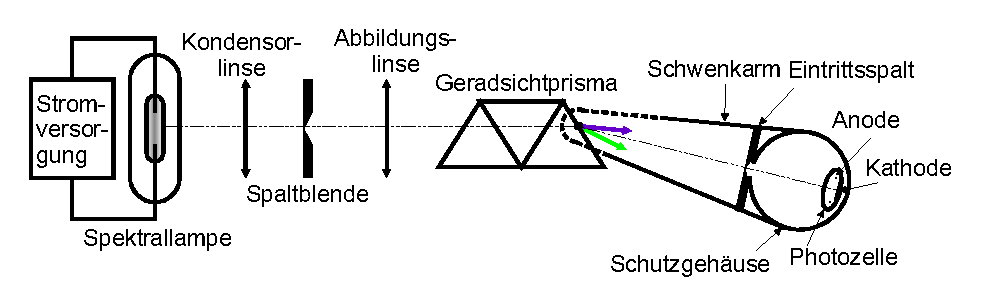
\includegraphics[width=\textwidth]{bilder/anordnung.pdf}
    \caption{Optische Konstruktion zur Herstellung von monochromatischem Licht. \cite{v500}}
    \label{fig:konstruktion}
\end{figure}

Dafür wird das von einer Hg-Spektrallampe ausgesendete polychromatische Licht durch Linsen und einem Spalt fokussiert.
Das Licht wird danach mit einem Prisma in monochromatische Spektrallinien bestimmter Wellenlängen zerlegt.
Die Photozelle kann dabei auf einem Schwenkarm so bewegt werden, 
dass die zu untersuchende Spektrallinie auf die Photokathode fällt.


\subsection{Messung des Photostroms}

Vor Beginn der Messung wird der Versuchsraum weitmöglichst vom Tageslicht und anderen Störfelder abgeschirmt.
Nach Ausrichten einer Spektrallinie auf die Photozelle wird diejenige Bremsspannung gesucht, 
bei der der Photostrom Null ist. 
Hiernach wird in $\qty{0.5}{\volt}$- bis $\qty{1.0}{\volt}$-Schritten die Spannung reduziert und der Photostrom notiert,
bis die Spannung null erreicht. Dies wird für die anderen erkennbaren Spektrallinien wiederholt.

Für die gelbe Spektrallinie wird zusätzlich die Spannung umgepolt 
und im negativem Spannungsbereich bis zu $\qty{-20}{\volt}$ gemessen.